\documentclass[10pt,a4paper]{article}

\usepackage[margin=22mm]{geometry}
\usepackage{amsmath,amssymb,mathtools}
\usepackage{booktabs,tabularx,array}
\usepackage{graphicx}
\usepackage{enumitem}
\usepackage{microtype}
\usepackage[hidelinks]{hyperref}

\newcommand{\Fm}{\boldsymbol{\mathcal F}}
\newcommand{\F}{\mathbf F}
\newcommand{\FE}{\mathbf F_{\!E}}
\newcommand{\FP}{\mathbf F_{\!P}}
\newcommand{\HP}{\mathbf H_{\!P}}
\newcommand{\HF}{\mathbf H_{\!F}}
\newcommand{\T}{\mathbf T}
\newcommand{\Ttotal}{\mathbf T_{\mathrm{total}}}
\newcommand{\old}{^{-}}
\newcommand{\new}{^{+}}

\setlist[itemize]{leftmargin=*,topsep=3pt,itemsep=2pt}
\setlength{\parindent}{0pt}
\setlength{\parskip}{4pt}

\title{\vspace{-1.2em}\textbf{Deformation History Through Reconnection}\\
\large Why direct full-gradient transport is preferable to $\Ttotal$}
\author{Technical note for the MTS2D reconnection model}
\date{\today}

\begin{document}
\maketitle
\vspace{-1.2em}

\section{Two different histories}

For the currently selected local reference triangle,
\begin{equation}
  \F=\FE\FP .
\end{equation}
The existing plastic history is
\begin{equation}
  \T=\FP\HP,
  \qquad
  \Ttotal:=\FE\T=\F\HP .
\end{equation}
At a flip, the update
\begin{equation}
  \HP\new=(\FP\new)^{-1}\FP\old\HP\old
\end{equation}
preserves the plastic branch exactly, $\T\new=\T\old$.  The reconstructed full
quantity is not preserved:
\begin{equation}
  \boxed{
  \Ttotal\new-\Ttotal\old
  =(\FE\new-\FE\old)\T\old .}
  \label{eq:t-total-change}
\end{equation}
This is appropriate if $\T$ is interpreted only as plastic bookkeeping.  It is
problematic if $\Ttotal$ is interpreted as the total deformation experienced
by the material, because a refreshed local elastic factor can modify previously
stored deformation.

Direct transport instead defines
\begin{equation}
  \Fm=\F\HF,
  \qquad
  \HF\new=(\F\new)^{-1}\F\old\HF\old .
  \label{eq:full-update}
\end{equation}
Therefore
\begin{equation}
  \boxed{\Fm\new=\F\new\HF\new
  =\F\old\HF\old=\Fm\old .}
\end{equation}

The mesh still selects a new local square reference after reconnecting; the
original triangle is not retained as the working reference of $\F$.  However,
$\HF$ accumulates the inverse changes of local reference.  Consequently,
$\Fm=\F\HF$ behaves exactly as if one original material reference had been kept
throughout.  Elastic and plastic deformation both remain in the total history,
while the constitutive energy may continue to use the refreshed local $\FE$.

\section{A decisive simple-shear check}

Consider a periodic cell with imposed simple shear
\begin{equation}
  \overline{\F}(\gamma)=
  \begin{pmatrix}1&\gamma\\0&1\end{pmatrix}.
\end{equation}
For a deformation $\mathbf y(\mathbf X)=\overline{\F}\mathbf X+\mathbf w$
with periodic $\mathbf w$, compatibility requires
\begin{equation}
  \left\langle\nabla_{\!X}\mathbf y\right\rangle
  =\overline{\F}+\left\langle\nabla_{\!X}\mathbf w\right\rangle
  =\overline{\F}.
  \label{eq:macro-compatibility}
\end{equation}
The periodic contribution averages to zero.  Thus any field interpreted as the
total deformation gradient from the original material reference must satisfy
\begin{equation}
  \langle F_{12}\rangle=\gamma,
  \qquad
  \langle F_{21}\rangle=0,
\end{equation}
regardless of internal plastic slips or edge flips.

In the $70\times70$ periodic test, both histories follow the imposed shear until
the intensive reconnection regime near $\gamma=0.72$.  At $\gamma=1$,
\begin{equation}
 \left\langle\Fm\right\rangle
 \simeq
 \begin{pmatrix}1.006&1.005\\-0.001&1.009\end{pmatrix},
 \qquad
 \left\langle\Ttotal\right\rangle
 \simeq
 \begin{pmatrix}0.957&0.335\\0.493&0.990\end{pmatrix}.
 \label{eq:final-means}
\end{equation}
The direct history reproduces the imposed map to about one percent.
$\Ttotal$, by contrast, loses two thirds of the imposed $12$ shear and develops
a large $21$ component that is absent from the boundary deformation.  This is
not a different mechanical response: $\Fm$ was passive, so both fields were
measured on the same simulation trajectory.  The discrepancy is entirely a
difference in history interpretation.

\begin{figure}[ht]
  \centering
  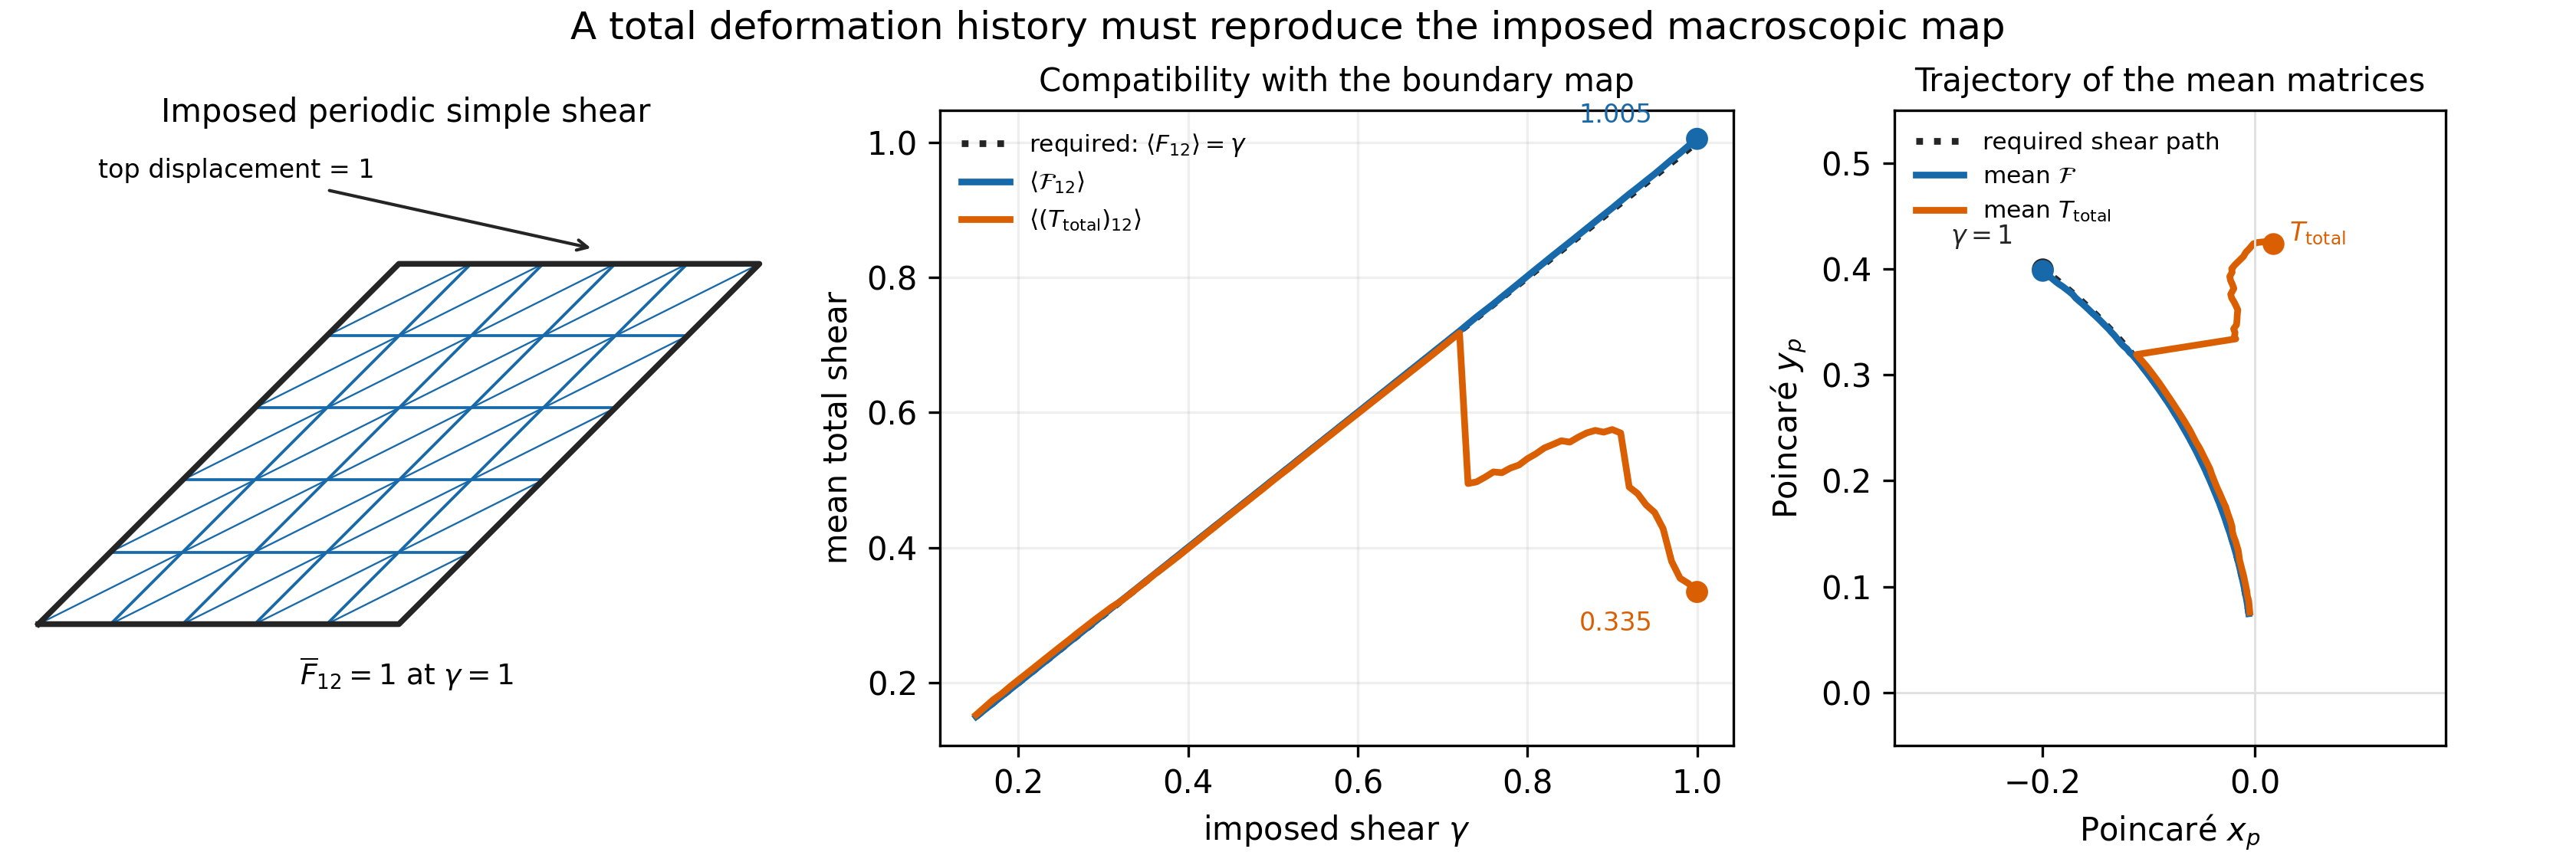
\includegraphics[width=0.95\linewidth]{../simple_shear_70_comparison/macroscopic_compatibility_example.png}
  \caption{Macroscopic compatibility provides an objective comparison.  The
  center panel shows that $\langle\Fm_{12}\rangle$ follows the imposed shear,
  while $\langle(\Ttotal)_{12}\rangle$ turns away after intensive reconnecting.
  The right panel shows the same result in the Poincar\'e disk: the trajectory
  of the mean $\Fm$ remains on the required pure-shear path, whereas the mean
  $\Ttotal$ leaves it.}
  \label{fig:compatibility}
\end{figure}

\section{Advantages and limitations}

{\small\hbadness=10000
\renewcommand{\arraystretch}{1.08}
\begin{tabularx}{\linewidth}{@{}>{\raggedright\arraybackslash}p{0.19\linewidth}
  >{\raggedright\arraybackslash}X >{\raggedright\arraybackslash}X@{}}
\toprule
 & \textbf{Plastic reconstruction $\Ttotal$} &
   \textbf{Direct history $\Fm$} \\
\midrule
Exactly preserved & Plastic branch $\T$. & Total gradient $\Fm$. \\
Effective reference & Refreshed $\FE$ combined with the stored plastic branch. &
Original material reference carried implicitly by $\HF$. \\
Elastic deformation & Only the current local elastic factor is included. &
All accumulated elastic and plastic deformation is retained. \\
After many flips & Components can be reinterpreted through
Equation~\eqref{eq:t-total-change}. & Unchanged by the flip itself; changes only
with subsequent physical deformation. \\
Simple-shear result & Violates the imposed macroscopic deformation when read as
a total gradient. & Satisfies the macroscopic compatibility condition. \\
Best use & $\T$ remains valuable for identifying plastic slips, but
$\Ttotal$ should not be used as total material history. & Primary total-history
field for output, trajectories, and Poincar\'e analysis. \\
\bottomrule
\end{tabularx}
\par}

Both approaches still require a rule assigning the histories of two parent
triangles to the two children created by an edge flip.  That remeshing choice is
shared and is not a reason to prefer either formula.  The relevant distinction
is what is preserved once the parent-child pairing has been chosen: only
$\Fm$ preserves the complete deformation history.

\section{Recommendation}

Use $\Fm=\F\HF$ as the total deformation-history field, while retaining the
existing local reduction and $\FE$ in the constitutive energy.  Keep $\T$ as the
plastic diagnostic.  Then $\FE$ means current recoverable deformation, $\T$
means accumulated plastic lattice branch, and $\Fm$ means total deformation
from the effective original material reference.  The closest square reference
remains a good local gauge, but the reported total history no longer depends on
which square candidate is selected at a flip.

\end{document}
